%%%%%%%%%%%%%%%%%%%%%%%%%%%%%%%%%%%%%%%%%
% Beamer Presentation
% LaTeX Template
% Version 1.0 (10/11/12)
%
% This template has been downloaded from:
% http://www.LaTeXTemplates.com
%
% License:
% CC BY-NC-SA 3.0 (http://creativecommons.org/licenses/by-nc-sa/3.0/)
%
%%%%%%%%%%%%%%%%%%%%%%%%%%%%%%%%%%%%%%%%%

%----------------------------------------------------------------------------------------
%	PACKAGES AND THEMES
%----------------------------------------------------------------------------------------

\documentclass[UTF8,aspectratio=169,14pt]{ctexbeamer}

\usepackage{hyperref}
\hypersetup{
	colorlinks=true,
	linkcolor=red,
	anchorcolor=blue,
	citecolor=green
}

\mode<presentation> {
	
	% The Beamer class comes with a number of default slide themes
	% which change the colors and layouts of slides. Below this is a list
	% of all the themes, uncomment each in turn to see what they look like.
	
	%\usetheme{default}
	%\usetheme{AnnArbor}
	%\usetheme{Antibes}
	%\usetheme{Bergen}
	%\usetheme{Berkeley}
	%\usetheme{Berlin}
	%\usetheme{Boadilla}
	%\usetheme{CambridgeUS}
	%\usetheme{Copenhagen}
	%\usetheme{Darmstadt}
	%\usetheme{Dresden}
	%\usetheme{Frankfurt}
	%\usetheme{Goettingen}
	%\usetheme{Hannover}
	%\usetheme{Ilmenau}
	%\usetheme{JuanLesPins}
	%\usetheme{Luebeck}
	\usetheme{Madrid}
	%\usetheme{Malmoe}
	%\usetheme{Marburg}
	%\usetheme{Montpellier}
	%\usetheme{PaloAlto}
	%\usetheme{Pittsburgh}
	%\usetheme{Rochester}
	%\usetheme{Singapore}
	%\usetheme{Szeged}
	%\usetheme{Warsaw}
	
	% As well as themes, the Beamer class has a number of color themes
	% for any slide theme. Uncomment each of these in turn to see how it
	% changes the colors of your current slide theme.
	
	%\usecolortheme{albatross}
	%\usecolortheme{beaver}
	%\usecolortheme{beetle}
	%\usecolortheme{crane}
	%\usecolortheme{dolphin}
	%\usecolortheme{dove}
	%\usecolortheme{fly}
	%\usecolortheme{lily}
	%\usecolortheme{orchid}
	%\usecolortheme{rose}
	%\usecolortheme{seagull}
	%\usecolortheme{seahorse}
	%\usecolortheme{whale}
	%\usecolortheme{wolverine}
	
	%\setbeamertemplate{footline} % To remove the footer line in all slides uncomment this line
	%\setbeamertemplate{footline}[page number] % To replace the footer line in all slides with a simple slide count uncomment this line
	
	%\setbeamertemplate{navigation symbols}{} % To remove the navigation symbols from the bottom of all slides uncomment this line
}

\usepackage{graphicx} % Allows including images
\graphicspath{{./figs/}}
\usepackage{booktabs} % Allows the use of \toprule, \midrule and \bottomrule in tables
\usepackage{longtable}
\usepackage{listings}
\usepackage{xcolor}
\lstset{numbers=left, %设置行号位置
	numberstyle=\tiny, %设置行号大小
	keywordstyle=\color{blue}, %设置关键字颜色
	commentstyle=\color[cmyk]{1,0,1,0}, %设置注释颜色
	frame=single, %设置边框格式
	escapeinside=``, %逃逸字符(1左面的键),用于显示中文
	%breaklines, %自动折行
	extendedchars=false, %解决代码跨页时,章节标题,页眉等汉字不显示的问题
	xleftmargin=2em,xrightmargin=2em, aboveskip=1em, %设置边距
	tabsize=4, %设置tab空格数
	showspaces=false %不显示空格
}
% Fonts
% \usepackage{libertine}
% \setmonofont{Courier}
\setCJKsansfont[ItalicFont=Noto Serif CJK SC Black, BoldFont=Noto Sans CJK SC Black]{Noto Sans CJK SC}


%----------------------------------------------------------------------------------------
% TITLE PAGE
%----------------------------------------------------------------------------------------

\title[第21讲]{第二十一讲 :分布式系统} % The short title appears at the bottom of every slide, the full title is only on the title page
\subtitle{第1节:分布式系统概述}
\author{向勇、陈渝、李国良} % Your name
\institute[清华大学] % Your institution as it will appear on the bottom of every slide, may be shorthand to save space
{
    清华大学计算机系 \\ % Your institution for the title page
    \medskip
    \textit{xyong,yuchen,liguoliang@tsinghua.edu.cn} % Your email address
}
\date{\today} % Date, can be changed to a custom date

\begin{document}
    
    \begin{frame}
        \titlepage % Print the title page as the first slide
    \end{frame}
    
    %----------------------------------------------
    \begin{frame}
        \frametitle{提纲} % Table of contents slide, comment this block out to remove it
        \tableofcontents % Throughout your presentation, if you choose to use \section{} and \subsection{} commands, these will automatically be printed on this slide as an overview of your presentation
        
        %% itemize
        %Ref:
        %    \begin{itemize}
        %        \item \href{http://osq.cs.berkeley.edu/public/JFoster-Drivers.ppt}{Linux Device Drivers Overview}
        %        \item \href{http://ermak.cs.nstu.ru/understanding.linux.kernel.pdf}{Understanding the Linux Kernel}
        %    \end{itemize}
        
    \end{frame}
    %----------------------------------------------
    %%  PRESENTATION SLIDES
    %----------------------------------------------
    \section{第1节:分布式系统概述} % Sections can be created in order to organize your presentation into discrete blocks, all sections and subsections are automatically printed in the table of contents as an overview of the talk
    %----------------------------------------------
    \subsection{通信基础} % A subsection can be created just before a set of slides with a common theme to further break down your presentation into chunks
    %----------------------------------------------
    \begin{frame}[fragile]
        \frametitle{通信基础}
        分布式系统改变了世界的面貌
        
        关键问题:  如何构建在组件故障时仍能工作的系统 
        
        
        
        %    \framesubtitle{xxxx}
        %% figure
            \begin{figure}
            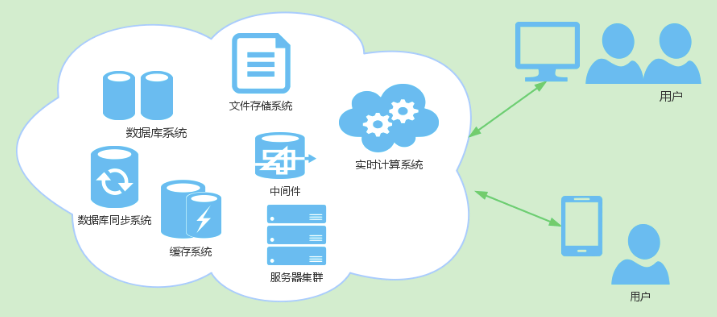
\includegraphics[width=0.8\linewidth]{figs/distributed.png}
          %  \caption{xxxx}
            \end{figure}
    \end{frame}
%----------------------------------------------
\begin{frame}[fragile]
    \frametitle{通信基础}
    %    \framesubtitle{xxxx}
    不可靠的通信层
    \begin{itemize}
        \item 现代网络的核心原则是,通信基本是不可靠的。
        \item 丢包是网络的基本现象
        \item 应该如何处理丢包?
    \end{itemize}
    %    \begin{figure}
    %        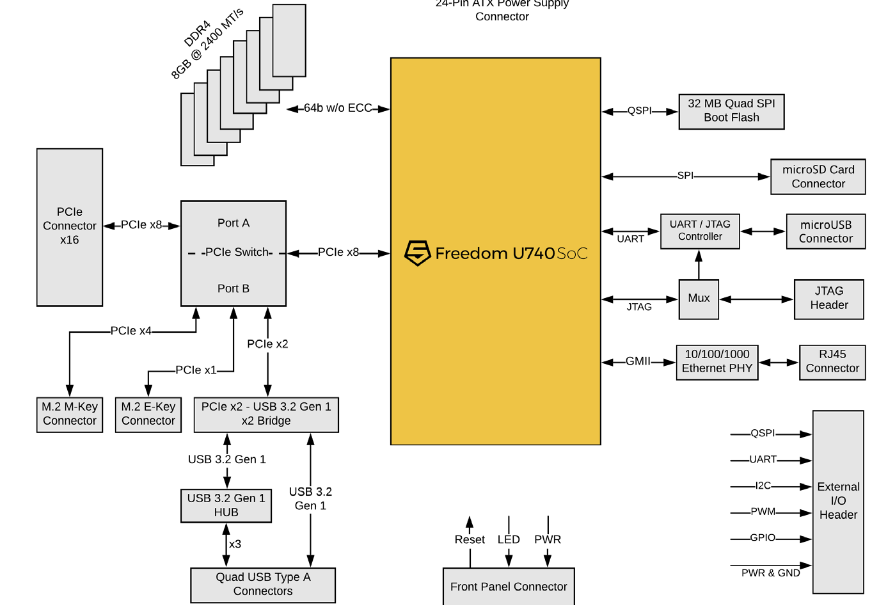
\includegraphics[width=0.3\linewidth]{figs/u740-arch.png}
    %        %  \caption{xxxx}
    %    \end{figure}
\end{frame}
%----------------------------------------------
\begin{frame}[fragile]
    \frametitle{通信基础}
%    \framesubtitle{xxxx}
一个基于UDP/IP构建的简单客户端
            \begin{figure}
    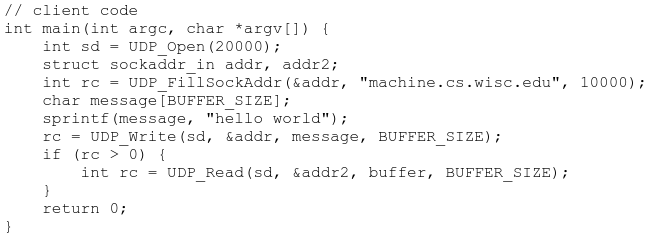
\includegraphics[width=1.\linewidth]{figs/udp-client.png}
    %  \caption{xxxx}
\end{figure}
\end{frame}

%----------------------------------------------
\begin{frame}[fragile]
    \frametitle{通信基础}
    %    \framesubtitle{xxxx}
    一个基于UDP/IP构建的简单服务器
    \begin{figure}
        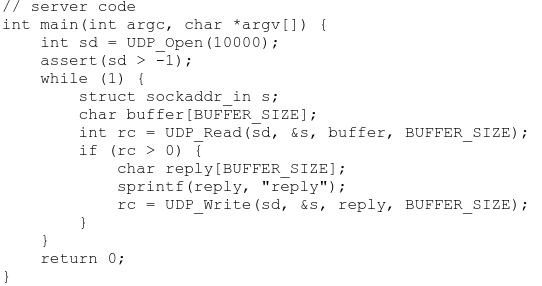
\includegraphics[width=0.8\linewidth]{figs/udp-server.png}
        %  \caption{xxxx}
    \end{figure}
\end{frame}
%----------------------------------------------
%----------------------------------------------
\begin{frame}[fragile]
    \frametitle{可靠的通信层}
    %    \framesubtitle{xxxx}
    问题:发送方如何知道接收方实际收到了消息? \pause
    \begin{itemize}
        \item 确认(ack, acknowledgment)
        \item 首先发送方向接收方发送消息,然后接收方发回确认
    \end{itemize}
    
    \begin{figure}
        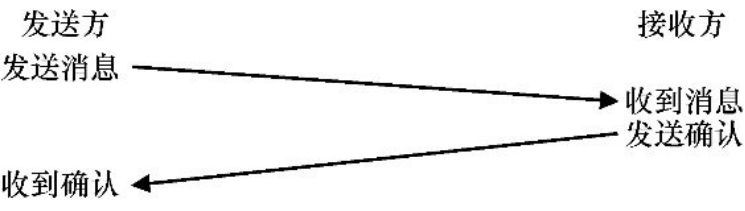
\includegraphics[width=0.8\linewidth]{figs/ack.png}
        \caption{消息加确认}
    \end{figure}
\end{frame}
%----------------------------------------------
\begin{frame}[fragile]
    \frametitle{可靠的通信层}
    %    \framesubtitle{xxxx}
    问题:如果没有收到确认,发送方应该怎么办?\pause
    \begin{itemize}
        \item 超时(timeout) + 重试(retry)
        \item 当发送方发送消息后,如在一定时间内未收到确认,则断定该消息已丢失
        \item 然后发送方就重试(retry)发送,再次发送相同的消息,希望这次能送达
    \end{itemize}

    \begin{figure}
        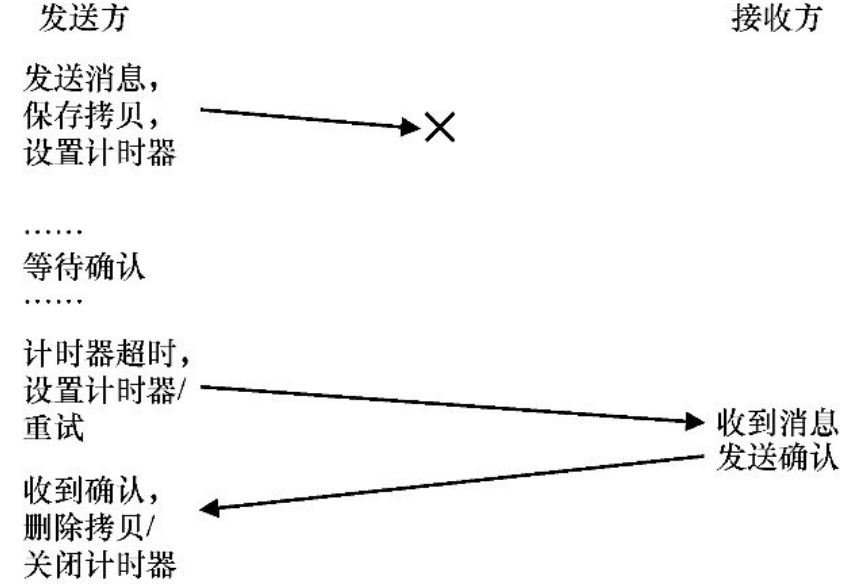
\includegraphics[width=0.4\linewidth]{figs/timeout.png}
          \caption{消息加确认:丢失的请求}
    \end{figure}
\end{frame}


%----------------------------------------------
\begin{frame}[fragile]
    \frametitle{可靠的通信层}
    %    \framesubtitle{xxxx}
    问题:如果没有收到确认,发送方应该怎么办?\pause
    \begin{itemize}
        \item 超时(timeout) + 重试(retry)
        \item 当发送方发送消息后,如在一定时间内未收到确认,则断定该消息已丢失
        \item 然后发送方就重试(retry)发送,再次发送相同的消息,希望这次能送达
    \end{itemize}
    
    \begin{figure}
        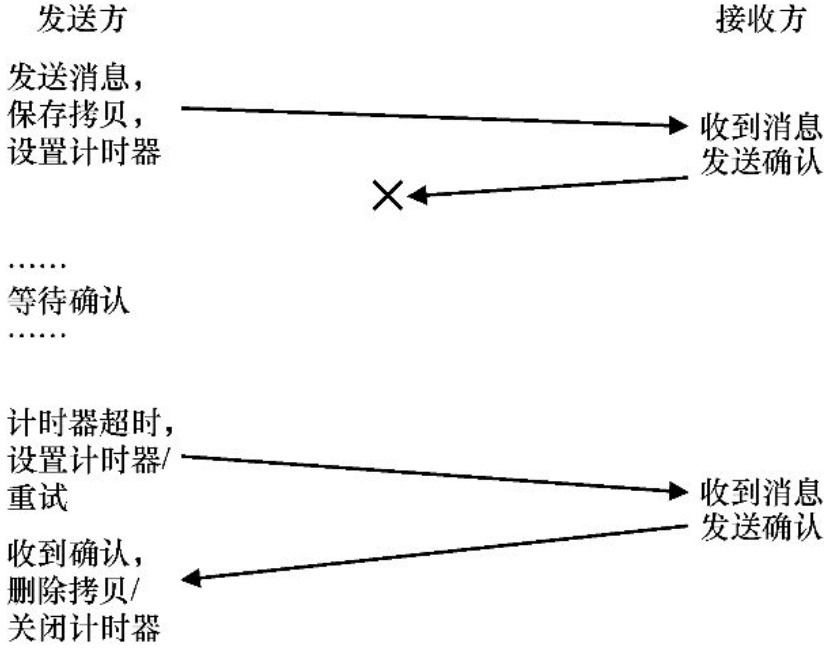
\includegraphics[width=0.35\linewidth]{figs/timeout-answer.png}
        \caption{消息加确认:丢失回答}
    \end{figure}
\end{frame}
%----------------------------------------------

%----------------------------------------------
\begin{frame}[fragile]
    \frametitle{可靠的通信层}
    %    \framesubtitle{xxxx}
    问题:如何保证接收方每个消息只接收一次(exactly once)?\pause
    \begin{itemize}
        \item 发送方为每条消息生成唯一的ID,接收方追踪它所见过的每个ID
        \item  顺序计数器(sequence counter)
            \begin{itemize}
            \item 发送消息时,计数器的当前值(N)都作为消息ID与消息一起发送;发送消息后,发送方递增该值(到N + 1)。
            \item 接收方使用其计数器值,作为发送方传入消息的ID的预期值。如接收的消息ID(N)与接收方计数器匹配,则确认该消息,并将其传递给上层应用程序。接收方断定这是第一次收到此消息。然后接收方递增其计数器,并等待下一条消息。
            \item 如确认丢失,则发送方将超时,并重新发送消息N。这时接收方计数器为N+1,因此接收器知道它已接收到该消息。因此它会确认该消息,但不会将其传递给应用程序。
            \end{itemize}
    \end{itemize}
    
%    \begin{figure}
%        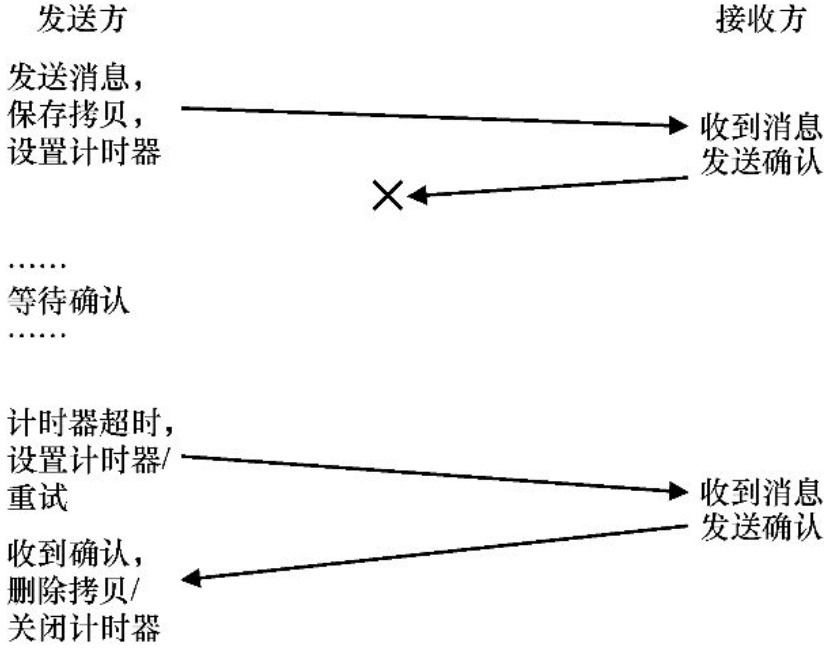
\includegraphics[width=0.35\linewidth]{figs/timeout-answer.png}
%        \caption{消息加确认:丢失回答}
%    \end{figure}
\end{frame}

%----------------------------------------------
\begin{frame}
    \frametitle{提纲} % Table of contents slide, comment this block out to remove it
    \tableofcontents % Throughout your presentation, if you choose to use \section{} and \subsection{} commands, these will automatically be printed on this slide as an overview of your presentation
    
    %% itemize
    %Ref:
    %    \begin{itemize}
    %        \item \href{http://osq.cs.berkeley.edu/public/JFoster-Drivers.ppt}{Linux Device Drivers Overview}
    %        \item \href{http://ermak.cs.nstu.ru/understanding.linux.kernel.pdf}{Understanding the Linux Kernel}
    %    \end{itemize}
    
\end{frame}
%----------------------------------------------
\subsection{通信抽象} % A subsection can be created just before a set of slides with a common theme to further break down your presentation into chunks
%----------------------------------------------
\begin{frame}[fragile]
    \frametitle{操作系统的通信抽象}
    %    \framesubtitle{xxxx}
    问题:有了基本的消息传递层,在构建分布式系统时,操作系统应该使用什么抽象通信?\pause
    \begin{itemize}
        \item 分布式共享内存(Distributed Shared Memory,DSM)
        \begin{itemize}
            \item 通过操作系统的虚拟内存系统,在不同机器上的进程间共享虚拟地址空间
        \end{itemize} \pause
            \item DSM的困难
        \begin{itemize}
            \item 故障问题
            \item 性能问题
        \end{itemize}
            \item 这种方法今天并未广泛使用
    \end{itemize}
    
%    \begin{figure}
%        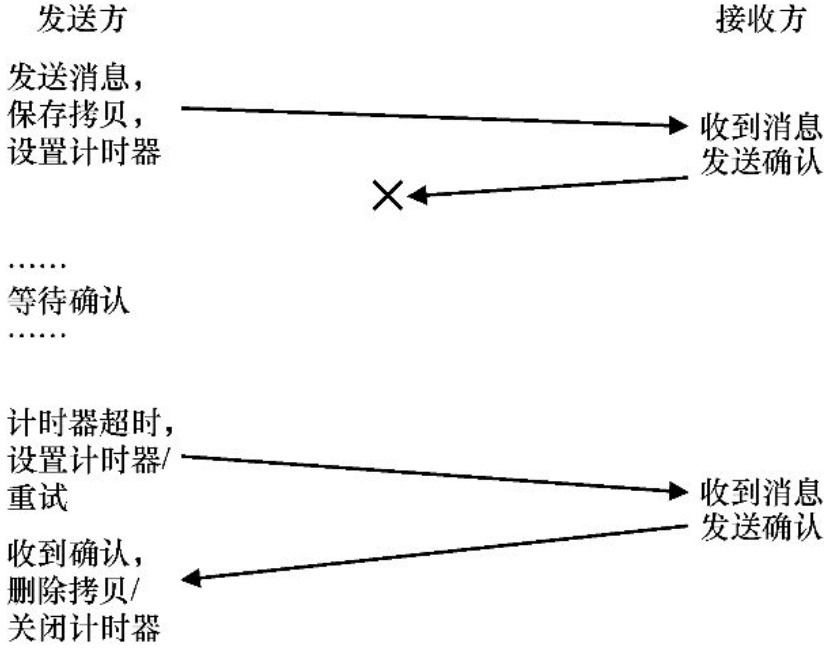
\includegraphics[width=0.35\linewidth]{figs/timeout-answer.png}
%        \caption{消息加确认:丢失回答}
%    \end{figure}
\end{frame}

%----------------------------------------------
\begin{frame}[fragile]
    \frametitle{编程语言的通信抽象}
    %    \framesubtitle{xxxx}
    问题:有了基本的消息传递层,在构建分布式系统时,编程语言应该使用什么抽象通信?
    \begin{itemize}
        \item 远程过程调用(RPC, Remote Procedure Call \pause
        \begin{itemize}
            \item 目标:像调用本地函数一样,在远程机器上执行代码
            \item RPC系统通常有两部分:
            \begin{itemize}
                \item  存根生成器(stub generator,也称协议编译器,protocol compiler)
                \item 运行时库(run-time library)
            \end{itemize}
        \end{itemize}
    \end{itemize}
    
    %    \begin{figure}
    %        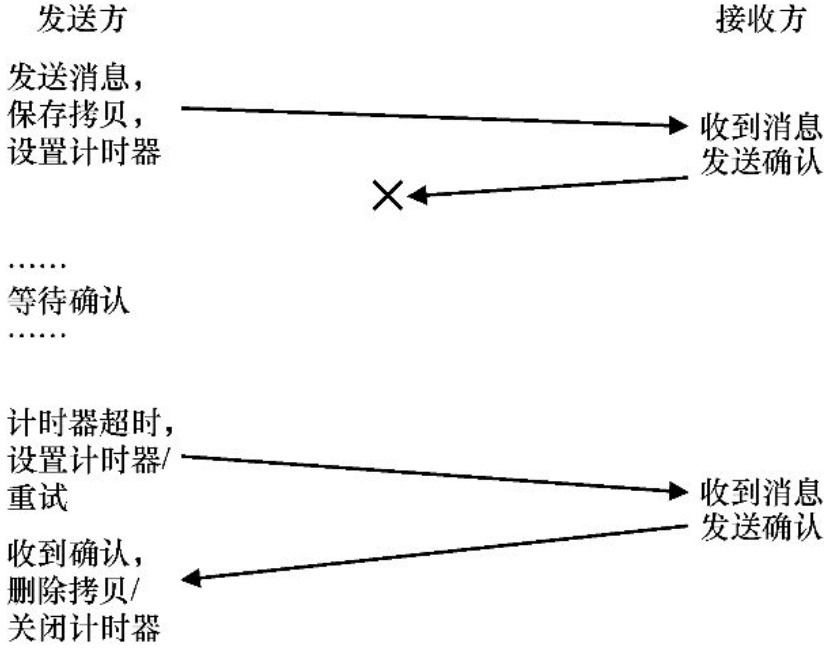
\includegraphics[width=0.35\linewidth]{figs/timeout-answer.png}
    %        \caption{消息加确认:丢失回答}
    %    \end{figure}
\end{frame}

%----------------------------------------------
\begin{frame}[fragile]
    \frametitle{存根生成器}
    %    \framesubtitle{xxxx}
存根生成器接受接口(interface)代码,并生成客户端存根(client stub)和服务端代理(server proxy)
    
        \begin{figure}
            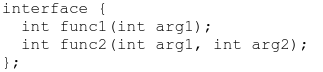
\includegraphics[width=0.6\linewidth]{figs/rpc-interface.png}
%            \caption{消息加确认:丢失回答}
        \end{figure}

    \begin{itemize}
        \item 客户端存根(client stub)
        \begin{itemize}
            \item 创建消息缓冲区,将所需信息打包到消息缓冲区中;
            \item 将消息发送到目标RPC服务器,等待回复;
            \item 解包返回代码和其他参数,返回调用函数。
        \end{itemize}
    \end{itemize}
    
\end{frame}

%----------------------------------------------
\begin{frame}[fragile]
    \frametitle{存根生成器}
    %    \framesubtitle{xxxx}
存根生成器接受接口(interface)代码,并生成客户端存根(client stub)和服务端代理(server proxy)
    
    \begin{figure}
        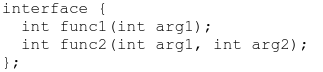
\includegraphics[width=0.6\linewidth]{figs/rpc-interface.png}
        %            \caption{消息加确认:丢失回答}
    \end{figure}
    \begin{itemize}
        \item 服务端代理(server proxy)
        \begin{itemize}
            \item 解包消息;
            \item 调用实际函数;
            \item 打包结果;发送回复。
        \end{itemize}
    \end{itemize}
    
\end{frame}

%----------------------------------------------
\begin{frame}[fragile]
    \frametitle{运行时库}
    %    \framesubtitle{xxxx}
    运行时库的作用
  
    \begin{itemize}
        \item 远程服务查找
        \item 构建RPC的传输层协议        
    \end{itemize}
\end{frame}

%----------------------------------------------
\begin{frame}[fragile]
    \frametitle{通信抽象中值得进一步思考的问题}

    \begin{itemize}
        \item 调用中的复杂参数,即一个包如何发送复杂的数据结构?
        \item 并发性的服务器组织方式?
        \item 当远程调用需要很长时间才能完成时,会发生什么?
        \item 是否向客户端暴露通信的异步性质,从而实现一些性能优化?
    \end{itemize}
\end{frame}
%----------------------------------------------
\end{document}
